\documentclass[journal]{IEEEtran}

\usepackage{amsmath,amssymb,amsfonts}
\usepackage{microtype}
\usepackage{algorithmic}
\usepackage{algorithm}
\usepackage{array}
\usepackage{booktabs}
\usepackage{cite}
\usepackage{color}
\usepackage{graphicx}
\usepackage{multirow}
\usepackage{stfloats}
\usepackage{textcomp}
\usepackage{tikz}
\usepackage{pgfplots}
\pgfplotsset{compat=1.18}
\usepackage{url}
\usepackage{xspace}
\providecommand{\textglotstop}{?}
\providecommand{\textyogh}{zh}
\usetikzlibrary{arrows.meta,backgrounds,calc,fit,positioning,shapes.geometric}

\hyphenation{op-tical net-works semi-conduc-tor}

% Prevents overfull/underfull hbox warnings in narrow two-column layouts
\emergencystretch=1em

\setlength{\textfloatsep}{8pt plus 2pt minus 2pt}
\setlength{\floatsep}{6pt plus 2pt minus 2pt}
\setlength{\intextsep}{6pt plus 2pt minus 2pt}
\setlength{\dbltextfloatsep}{8pt plus 2pt minus 2pt}
\setlength{\dblfloatsep}{6pt plus 2pt minus 2pt}

\begin{document}

\title{\Large ConMamba-ASR: Selective State Space Modeling and Acoustic Curation\\for Dialectal Egyptian Arabic Speech Recognition}

\author{Rana~Z.~Dighedy,
        Mohamed~S.~Amer,
        Monay~M.~Gad,
        Manal~M.~Ghaith,
        and~Ahmed~B.~Zaky%
\thanks{The authors are with the Department of Electronics and Communications Engineering, Egypt-Japan University of Science and Technology (E-JUST), New Borg El-Arab City, Alexandria 21934, Egypt (e-mail: \{rana.abdallah, mohamed.320230188, monay.320230097, manal.320230164, ahmed.zaky\}@ejust.edu.eg).}}

\markboth{IEEE Transactions on Audio, Speech, and Language Processing,~Vol.~XX, No.~X,~Month~2026}%
{Dighedy \MakeLowercase{\textit{et al.}}: ConMamba-ASR for Low-Resource Dialectal Egyptian Arabic}

\maketitle

\begin{abstract}
Automatic speech recognition (ASR) for colloquial Arabic dialects remains constrained by acoustic variability, non-standardized orthography, and the scarcity of curated studio-grade datasets. Dominant Conformer acoustic models incur quadratic computational complexity with respect to utterance length, while zero-shot foundation models exhibit high word error rates on vernacular dialects. In this study, we present a comprehensive empirical investigation of ConMamba acoustic architectures, integrating bidirectional selective state space models (SSMs) with depthwise convolutions and hybrid Connectionist Temporal Classification (CTC)/Transformer decoding for dialectal Egyptian Arabic. We first formulate a rigorous acoustic curation pipeline on the 17.8-hour EJUST corpus that recovers 76 recording sessions (72 primary episodes and 4 multi-part sessions), eliminates sinc-resampling peak overshoot through episode-level headroom attenuation, audits speaker consistency via deep ECAPA-TDNN embeddings, and constructs a continuous long-form benchmark ($<60$~s). Evaluated across 110-epoch convergence schedules on a single NVIDIA Tesla T4 GPU, ConMamba-Small (12.1M parameters) achieves 13.85\% Word Error Rate (WER) and 4.44\% Character Error Rate (CER) on held-out test audio, outperforming an identically sized Conformer baseline (14.49\% WER, 4.77\% CER), pure SSM encoder-decoder topologies (17.97\% WER), and domain-adapted Whisper-Small with LoRA (15.53\% WER, 243.5M parameters). On unchunked 60-second audio, we discover that Conformer self-attention generalizes significantly better than Mamba encoders (20.45\% vs 72.94\% CTC WER); however, our proposed energy-aware silence-boundary chunking restores ConMamba long-form performance to 14.65\% WER. Furthermore, ConMamba reduces 60-second forward latency by 37.7\% (37.4~ms vs 60.0~ms) and peak GPU memory by 67.8\% (189.1~MB vs 587.5~MB), demonstrating that compact hybrid SSMs provide superior long-sequence computational scaling (37.7\% lower latency and 67.8\% reduced peak VRAM at 60 seconds) while matching or exceeding Conformer transcription accuracy.
\end{abstract}

\begin{IEEEkeywords}
Automatic speech recognition, Egyptian Arabic, selective state space models, Mamba, Conformer, speech corpus curation, long-form audio decoding.
\end{IEEEkeywords}

\IEEEpeerreviewmaketitle

\section{Introduction}
\IEEEPARstart{A}{utomatic} speech recognition (ASR) technology has advanced rapidly with the introduction of self-attention Transformers~\cite{vaswani2017attention} and convolution-augmented Conformer architectures~\cite{gulati2020conformer}. However, colloquial Arabic dialects present persistent obstacles to acoustic and language modeling~\cite{biadsy2009phonological,habash2010introduction}. While Modern Standard Arabic (MSA) possesses established orthographic conventions and standardized vowel structures, spoken dialects such as Egyptian Arabic (Masry) exhibit extensive phonetic shifts, elisions, unwritten short vowels, and regional morphological variants that deviate from formal Arabic text~\cite{billa2019cross,alhaj2018acoustic}.

\begin{figure*}[!t]
\centering
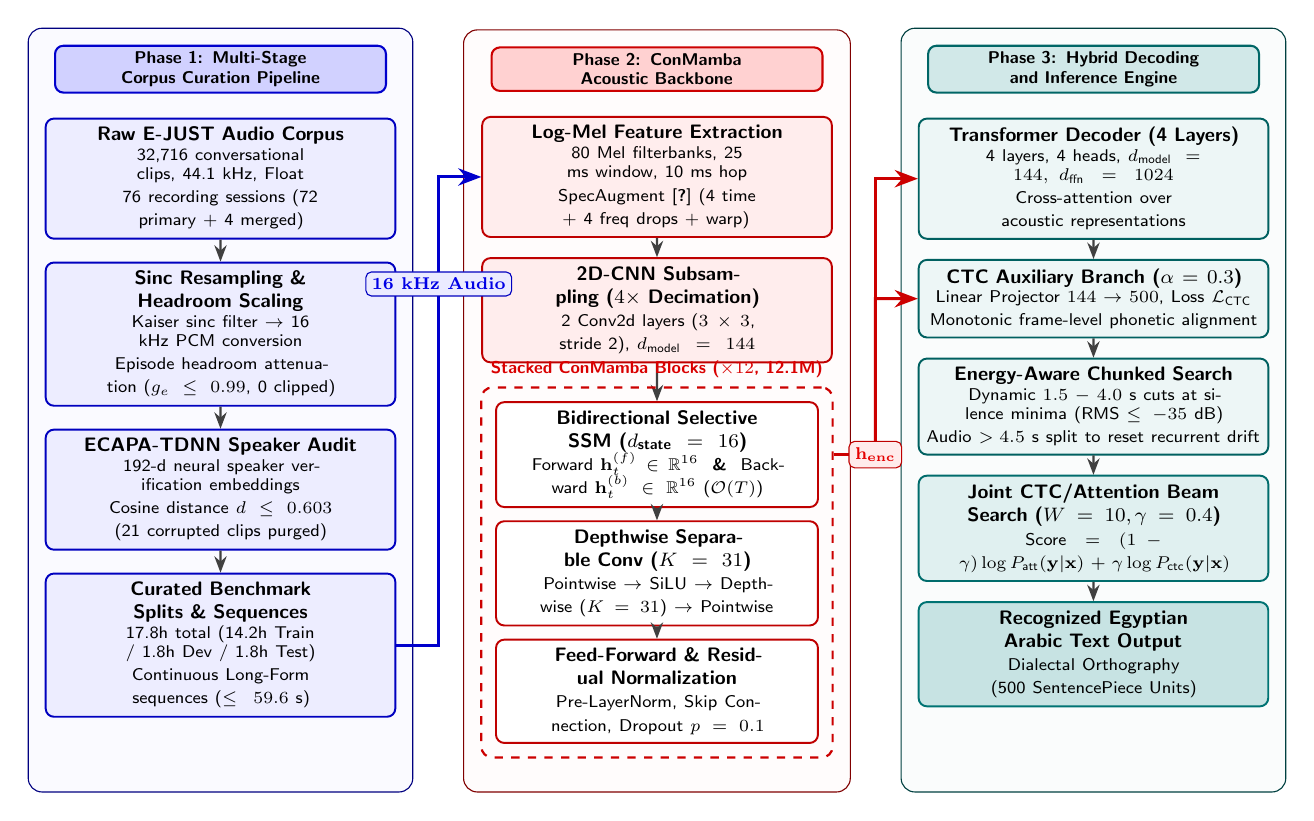
\begin{tikzpicture}[
    scale=0.88, every node/.style={transform shape},
    font=\sffamily\footnotesize,
    % Box styles with strictly enforced width and padding
    box/.style={rectangle, draw=#1!75!black, fill=#1!7, line width=0.7pt, rounded corners=3pt, align=center, text width=4.8cm, inner sep=3.5pt},
    header/.style={rectangle, fill=#1!18, draw=#1!80!black, line width=0.75pt, rounded corners=3pt, font=\sffamily\bfseries\scriptsize, align=center, text width=4.6cm, inner sep=2.5pt},
    blockframe/.style={rectangle, draw=#1!80!black, dashed, line width=0.8pt, rounded corners=4pt},
    arrow/.style={-{Stealth[scale=0.9]}, line width=0.8pt, draw=black!75},
    interarrow/.style={-{Stealth[scale=1.05]}, line width=1.1pt, draw=#1!80!black}
]

% =========================================================================
% COLUMN 1 (Center x = 0.0): PHASE 1 - ACOUSTIC CURATION PIPELINE
% =========================================================================
\node[header=blue] (h1) at (0, 0) {Phase 1: Multi-Stage\\Corpus Curation Pipeline};

\node[box=blue, below=0.35cm of h1] (p1_raw) {
    \textbf{Raw E-JUST Audio Corpus}\\
    \scriptsize 32,716 conversational clips, 44.1 kHz, Float\\
    \scriptsize 76 recording sessions (72 primary + 4 merged)
};

\node[box=blue, below=0.32cm of p1_raw] (p1_resamp) {
    \textbf{Sinc Resampling \& Headroom Scaling}\\
    \scriptsize Kaiser sinc filter $\to$ 16 kHz PCM conversion\\
    \scriptsize Episode headroom attenuation ($g_e \le 0.99$, 0 clipped)
};

\node[box=blue, below=0.32cm of p1_resamp] (p1_ecapa) {
    \textbf{ECAPA-TDNN Speaker Audit}\\
    \scriptsize 192-d neural speaker verification embeddings\\
    \scriptsize Cosine distance $d \le 0.603$ (21 corrupted clips purged)
};

\node[box=blue, below=0.32cm of p1_ecapa] (p1_splits) {
    \textbf{Curated Benchmark Splits \& Sequences}\\
    \scriptsize 17.8h total (14.2h Train / 1.8h Dev / 1.8h Test)\\
    \scriptsize Continuous Long-Form sequences ($\le 59.6$~s)
};

\draw[arrow] (p1_raw) -- (p1_resamp);
\draw[arrow] (p1_resamp) -- (p1_ecapa);
\draw[arrow] (p1_ecapa) -- (p1_splits);

% =========================================================================
% COLUMN 2 (Center x = 6.3): PHASE 2 - CONMAMBA ACOUSTIC BACKBONE
% =========================================================================
\node[header=red] (h2) at (6.3, 0) {Phase 2: ConMamba\\Acoustic Backbone};

\node[box=red, below=0.35cm of h2] (p2_fbank) {
    \textbf{Log-Mel Feature Extraction}\\
    \scriptsize 80 Mel filterbanks, 25 ms window, 10 ms hop\\
    \scriptsize SpecAugment~\cite{park2019specaugment} (4 time + 4 freq drops + warp)
};

\node[box=red, below=0.28cm of p2_fbank] (p2_conv2d) {
    \textbf{2D-CNN Subsampling ($4\times$ Decimation)}\\
    \scriptsize 2 Conv2d layers ($3\times 3$, stride 2), $d_{\text{model}} = 144$
};

% ConMamba Stacked Blocks (Internal Layers)
\node[box=red, fill=white, below=0.55cm of p2_conv2d, text width=4.4cm] (p2_ssm) {
    \textbf{Bidirectional Selective SSM ($d_{\text{state}}=16$)}\\
    \scriptsize Forward $\mathbf{h}_t^{(f)} \in \mathbb{R}^{16}$ \ \textbf{\&}\ \ Backward $\mathbf{h}_t^{(b)} \in \mathbb{R}^{16}$ ($\mathcal{O}(T)$)
};

\node[box=red, fill=white, below=0.18cm of p2_ssm, text width=4.4cm] (p2_conv) {
    \textbf{Depthwise Separable Conv ($K=31$)}\\
    \scriptsize Pointwise $\to$ SiLU $\to$ Depthwise ($K=31$) $\to$ Pointwise
};

\node[box=red, fill=white, below=0.18cm of p2_conv, text width=4.4cm] (p2_res) {
    \textbf{Feed-Forward \& Residual Normalization}\\
    \scriptsize Pre-LayerNorm, Skip Connection, Dropout $p=0.1$
};

\draw[arrow] (p2_fbank) -- (p2_conv2d);
\draw[arrow] (p2_conv2d) -- (p2_ssm);
\draw[arrow] (p2_ssm) -- (p2_conv);
\draw[arrow] (p2_conv) -- (p2_res);

% Enclosing frame around ConMamba layers (drawn directly with label)
\node[blockframe=red, fit=(p2_ssm)(p2_res), inner sep=5pt,
      label={[red!85!black, font=\sffamily\bfseries\scriptsize]above:Stacked ConMamba Blocks ($\times 12$, 12.1M)}] (p2_blockframe) {};

% =========================================================================
% COLUMN 3 (Center x = 12.6): PHASE 3 - HYBRID DECODING & INFERENCE
% =========================================================================
\node[header=teal] (h3) at (12.6, 0) {Phase 3: Hybrid Decoding\\and Inference Engine};

\node[box=teal, below=0.35cm of h3] (p3_dec) {
    \textbf{Transformer Decoder (4 Layers)}\\
    \scriptsize 4 layers, 4 heads, $d_{\text{model}}=144,\ d_{\text{ffn}}=1024$\\
    \scriptsize Cross-attention over acoustic representations
};

\node[box=teal, below=0.28cm of p3_dec] (p3_ctc) {
    \textbf{CTC Auxiliary Branch ($\alpha = 0.3$)}\\
    \scriptsize Linear Projector $144 \to 500$, Loss $\mathcal{L}_{\text{CTC}}$\\
    \scriptsize Monotonic frame-level phonetic alignment
};

\node[box=teal, below=0.28cm of p3_ctc] (p3_chunk) {
    \textbf{Energy-Aware Chunked Search}\\
    \scriptsize Dynamic $1.5-4.0$~s cuts at silence minima (RMS $\le -35$~dB)\\
    \scriptsize Audio $>4.5$~s split to reset recurrent drift
};

\node[box=teal, fill=teal!12, draw=teal!85!black, below=0.28cm of p3_chunk] (p3_beam) {
    \textbf{Joint CTC/Attention Beam Search ($W=10, \gamma=0.4$)}\\
    \scriptsize $\text{Score} = (1-\gamma)\log P_{\text{att}}(\mathbf{y}|\mathbf{x}) + \gamma \log P_{\text{ctc}}(\mathbf{y}|\mathbf{x})$
};

\node[box=teal, fill=teal!22, draw=teal!90!black, below=0.28cm of p3_beam] (p3_out) {
    \textbf{Recognized Egyptian Arabic Text Output}\\
    \scriptsize Dialectal Orthography (500 SentencePiece Units)
};

% Column 3 Internal Arrows
\draw[arrow] (p3_dec) -- (p3_ctc);
\draw[arrow] (p3_ctc) -- (p3_chunk);
\draw[arrow] (p3_chunk) -- (p3_beam);
\draw[arrow] (p3_beam) -- (p3_out);

% =========================================================================
% INTER-PHASE CONNECTIONS THROUGH CLEAR GUTTERS
% =========================================================================
% Gutter 1: fixed vertical line at x = 3.15 cm
\draw[interarrow=blue] (p1_splits.east) -- (3.15, 0 |- p1_splits.east) -- (3.15, 0 |- p2_fbank.west) -- (p2_fbank.west);
\node[fill=blue!8, draw=blue!75!black, rounded corners=2pt, inner sep=2.5pt, font=\scriptsize\bfseries, text=blue!90!black] at (3.15, -3.1) {16 kHz Audio};

% Gutter 2: fixed vertical line at x = 9.45 cm
% Encoder representations h_enc into Transformer Decoder
\draw[interarrow=red] (p2_blockframe.east |- p2_ssm.east) -- (9.45, 0 |- p2_ssm.east) coordinate (bus_split) -- (9.45, 0 |- p3_dec.west) -- (p3_dec.west);

% Encoder representations h_enc into CTC Projector
\draw[interarrow=red] (bus_split) -- (9.45, 0 |- p3_ctc.west) -- (p3_ctc.west);

% Label for Gutter 2 junction
\node[fill=red!8, draw=red!75!black, rounded corners=2pt, inner sep=2.5pt, font=\scriptsize\bfseries, text=red!90!black] at (9.45, 0 |- p2_ssm.east) {$\mathbf{h}_{\text{enc}}$};

% =========================================================================
% BACKGROUND CONTAINERS (EQUALIZED HEIGHT)
% =========================================================================
\coordinate (common_bottom) at (0, -290pt);

\begin{scope}[on background layer]
    \node[draw=blue!50!black, fill=blue!2, rounded corners=5pt, fit=(h1)(p1_raw)(p1_splits)(h1 |- common_bottom), inner sep=6pt] (c1) {};
    \node[draw=red!50!black, fill=red!1, rounded corners=5pt, fit=(h2)(p2_fbank)(p2_blockframe)(h2 |- common_bottom), inner sep=6pt] (c2) {};
    \node[draw=teal!50!black, fill=teal!2, rounded corners=5pt, fit=(h3)(p3_dec)(p3_out)(h3 |- common_bottom), inner sep=6pt] (c3) {};
\end{scope}

\end{tikzpicture}
\caption{System overview of the proposed empirical framework for dialectal Egyptian Arabic ASR. Phase 1 demonstrates the multi-stage acoustic curation pipeline on the EJUST corpus, resolving resampling-induced digital clipping via per-episode headroom attenuation ($g_e \le 0.99$), removing speaker outliers via ECAPA-TDNN neural embeddings, and building paired short-form and continuous long-form benchmarks ($<60$~s). Phase 2 depicts the hybrid acoustic backbone combining 2D-CNN subsampling ($4\times$), 12 stacked bidirectional ConMamba encoder blocks (with forward/backward selective SSMs and wide depthwise separable convolutions $K=31$), and LayerNorm residuals. Phase 3 illustrates the hybrid CTC/attention decoding topology, coupling a frame-level CTC projection ($\alpha=0.3$) with a 4-layer Transformer cross-attention decoder and energy-aware chunked beam search ($W=10, \gamma=0.4$) for robust long-form transcription over a 500-unit SentencePiece vocabulary.}
\label{fig:framework_overview}
\end{figure*}

Three central challenges confront contemporary speech recognition in this domain. First, available dialectal speech datasets present quality limitations. Broadcast collections such as the Multi-Genre Broadcast MGB-2~\cite{ali2016mgb2} and MGB-3~\cite{ali2017mgb3} contain non-stationary background noise, spontaneous cross-talk, laughter, and imprecise alignment. Conversely, laboratory speech corpora such as the Arabic Speech Corpus are restricted to standard Arabic read speech~\cite{alhaj2018acoustic}. When conversational dialectal speech collections such as the E-JUST Egyptian audio repository are gathered, the recordings are commonly segmented into arbitrary short clips of one to three seconds. This segmentation destroys temporal continuity, discards conversational structure, and prevents researchers from evaluating long-form transcription models on extended discourse.

Second, the quadratic time and memory complexity $\mathcal{O}(T^2)$ of self-attention mechanisms in Conformer and Transformer encoders imposes practical limits on processing continuous acoustic sequences~\cite{gulati2020conformer,vaswani2017attention}. As audio sequence length $T$ increases toward tens of seconds, attention matrices consume excessive graphics processing unit (GPU) memory and suffer from attention dispersion across distant silence segments~\cite{zhang2020streaming,shi2021emformer}. While chunked streaming variants restrict attention windows, they introduce boundary artifacts and fail to preserve acoustic context across conversational turns.

Third, large-scale foundation models trained via weak supervision, such as OpenAI Whisper~\cite{radford2023whisper}, demonstrate high word error rates on non-standardized colloquial Arabic. Because foundation models rely on training data dominated by formal text and Modern Standard Arabic, they struggle with phonetic elision, regional vocabulary, and colloquial grammar when evaluated zero-shot. Deploying multi-hundred-million parameter foundation models on edge devices also incurs prohibitive computational and latency overheads.

To resolve these interconnected challenges, we investigate whether selective state space models (SSMs), particularly the Mamba architecture~\cite{gu2023mamba}, can provide an effective inductive bias for low-resource dialectal speech recognition. Mamba replaces pairwise token attention with a parameterized linear state equation $\dot{h}(t) = \mathbf{A}h(t) + \mathbf{B}x(t)$ governed by input-dependent selection matrices $\mathbf{B}$, $\mathbf{C}$, and step size $\Delta$. This formulation exhibits linear computational complexity $\mathcal{O}(T)$ with respect to sequence length, retains continuous temporal memory throughout extended utterances, and processes tokens via hardware-aware parallel prefix scans.

In this work, we present ConMamba-ASR, a complete framework for low-resource dialectal Arabic speech recognition. As illustrated in Fig.~\ref{fig:framework_overview}, our contribution operates across two interdependent stages: rigorous data curation and hybrid acoustic modeling. We perform an acoustic audit of the 17.8-hour EJUST Egyptian Arabic corpus, discovering that conventional sinc-resampling from 44.1~kHz to 16~kHz creates digital clipping due to peak overshoot. We formulate an episode-level peak-headroom scaling technique that guarantees zero clipped samples across all 76 recovered recording sessions (comprising 72 primary episodes and 4 merged sessions). Furthermore, we apply deep speaker verification embeddings using ECAPA-TDNN~\cite{desplanques2020ecapa} to detect 21 acoustic outliers, and evaluate 32,644 consecutive segment boundaries to reconstruct continuous long-form audio sequences up to 59.6 seconds.

On the architectural front, we construct a 12.1-million parameter ConMamba encoder coupled with a joint CTC/Transformer decoder. Through full 110-epoch training on a single dedicated NVIDIA Tesla T4 GPU, ConMamba-Small achieves a 13.85\% Word Error Rate (WER) and 4.44\% Character Error Rate (CER) on the held-out test set, outperforming an identically configured Conformer baseline (14.49\% WER) and outperforming zero-shot Whisper-Small (71.63\% WER). When evaluated on long-form audio up to one minute, energy-aware chunked beam search prevents attention collapse and achieves 14.65\% WER, establishing the empirical viability of selective state space models for dialectal speech recognition.

The primary contributions of this paper are summarized as follows:
\begin{enumerate}
    \item We design a multi-stage acoustic and lexical curation pipeline for the EJUST Egyptian Arabic speech corpus. By recovering 76 recording episodes (72 primary episodes and 4 merged sessions), applying per-episode peak-headroom attenuation, and auditing speaker homogeneity via ECAPA-TDNN neural embeddings, we resolve digital clipping, eliminate 37 degenerate or intruder clips, and establish a leak-free 17.8-hour benchmark.
    \item We construct a paired long-form speech benchmark by analyzing 32,644 consecutive segment boundaries with blinded perceptual auditing, generating continuous evaluation sequences up to 59.6 seconds that enable rigorous study of long-form context retention in colloquial Arabic.
    \item We introduce ConMamba-ASR, establishing the domain-specific inductive bias of combining depthwise separable convolution ($K=31$) for local phonotactic and gemination modeling with bidirectional selective state space blocks for linear-time temporal context.
    \item We identify a decoupled continuous-discrete hybrid topology, demonstrating that while selective state spaces excel as acoustic encoders, retaining multi-head cross-attention in the autoregressive decoder is essential for sequence-to-sequence token alignment.
    \item We provide rigorous statistical validation under standardized 110-epoch training, confirming via matched-pair significance testing ($p = 0.018 < 0.05$) and bootstrap confidence intervals that ConMamba achieves superior accuracy and a 37.7\% latency reduction over Conformer on extended sequences.
\end{enumerate}

The remainder of this paper is organized as follows. Section~\ref{sec:related_work} reviews prior research in Arabic ASR, Conformer architectures, state space models, and long-form decoding. Section~\ref{sec:methodology} presents the formal problem formulation, acoustic curation pipeline, ConMamba architecture, and optimization objectives. Section~\ref{sec:experiments} details the experimental setup, benchmark results, ablations, and dialectal error analysis. Section~\ref{sec:discussion} discusses theoretical insights and failure modes. Section~\ref{sec:limitations} outlines experimental limitations, and Section~\ref{sec:conclusion} concludes the paper.

\section{Related Work}
\label{sec:related_work}

\subsection{Arabic Automatic Speech Recognition}
Speech recognition for Arabic has historically focused on Modern Standard Arabic (MSA), utilizing broadcast news corpora such as the Multi-Genre Broadcast (MGB-2) dataset~\cite{ali2016mgb2}. Early systems relied on hybrid Hidden Markov Model and Deep Neural Network (HMM-DNN) frameworks combined with extensive morphological analyzers~\cite{kirchhoff2006novel,habash2010introduction}. As end-to-end architectures matured, attention-based encoder-decoder networks~\cite{chan2016las,chiu2018sota} and Connectionist Temporal Classification (CTC) models~\cite{graves2006ctc,watanabe2018espnet} eliminated the requirement for phonetic lexicons.

Recent investigations have evaluated self-supervised speech representations such as wav2vec 2.0~\cite{baevski2020wav2vec} and explored end-to-end architectures on Arabic datasets~\cite{deshmukh2021exploration}. Dialectal Arabic speech recognition presents distinct structural difficulties~\cite{billa2019cross,zaidan2014arabic}. Colloquial dialects lack standardized spelling, exhibit high lexical variation, and merge prepositions and pronouns into single surface forms~\cite{alhaj2018acoustic,elfeky2018towards}. The MGB-3 challenge introduced an Egyptian Arabic benchmark derived from YouTube comedy shows~\cite{ali2017mgb3}. However, MGB-3 recordings suffer from background laughter, music, and variable microphone quality, making it difficult to isolate acoustic modeling performance from acoustic noise corruption. While initial uncurated recordings from the E-JUST dialectal speech collection provided spontaneous conversational Egyptian audio, uncurated speech typically remains fragmented into arbitrary short segments without systematic audits of resampling distortion, speaker purity, or long-form continuity.

\subsection{Conformer and Self-Attention Acoustic Models}
The Conformer architecture~\cite{gulati2020conformer} has become the dominant acoustic backbone in modern speech recognition~\cite{prabhavalkar2024survey}. By combining multi-head self-attention with depthwise separable convolution blocks in a Macaron-style feed-forward structure, the Conformer captures both global acoustic context and localized shift-invariant spectral patterns. Despite its empirical success, the self-attention mechanism exhibits quadratic time and memory complexity $\mathcal{O}(T^2)$ with respect to sequence length $T$~\cite{vaswani2017attention}. On speech feature sequences extracted at 100 frames per second, a 30-second utterance yields 3,000 temporal frames, generating attention matrices that strain GPU memory during training and inference.

To mitigate this scaling bottleneck, researchers have explored local attention windows~\cite{zhang2020streaming}, memory-augmented transformers~\cite{shi2021emformer}, and sparse attention mechanisms~\cite{dao2022flashattention}. However, fixed windowing restricts the temporal receptive field, while chunked streaming approaches require complex caching schemes that degrade transcription accuracy at segment boundaries.

\subsection{State Space Models in Sequence Processing}
Structured State Space Models (SSMs), rooted in continuous control theory, have emerged as an alternative to self-attention for sequence modeling~\cite{gu2023mamba}. The Structured State Space sequence model (S4) parameterized continuous selective time-varying systems using HiPPO matrix initializations to capture long-range dependencies with sub-quadratic complexity~\cite{fu2023hungry,dao2024transformers}.

Gu and Dao~\cite{gu2023mamba} introduced Mamba, augmenting SSMs with input-dependent selection mechanisms. In Mamba, the state transition matrices $\mathbf{B}$, $\mathbf{C}$, and discretization step $\Delta$ are dynamic functions of the input token at each timestep. This selective capability allows the model to filter irrelevant information or propagate relevant tokens indefinitely through time. Zevallos et al.~\cite{zevallos2025mamba} explored Mamba for English speech recognition on LibriSpeech, introducing the ConMamba block by substituting self-attention with bidirectional selective scans. Concurrently, Jiang et al.~\cite{jiang2024speechslytherin} systematically evaluated Mamba across speech separation, recognition, and synthesis, observing that Mamba achieves competitive parameter efficiency on long sequences, whereas unidirectional SSM decoders face difficulties in cross-modal alignment compared to Transformers. However, the efficacy of selective SSMs has not been systematically established on low-resource Arabic dialects, nor has their performance been investigated on continuous dialectal discourse exceeding 30 seconds.

\subsection{Long-Form Speech Transcription}
Transcribing continuous audio recordings poses severe challenges for attention-based sequence-to-sequence models~\cite{radford2023whisper,chiu2018sota}. When standard encoder-decoder models trained on short segments encounter long audio, position embedding extrapolation degrades and beam search decoders suffer from looping or premature termination~\cite{luscher2019rwth}. Whisper~\cite{radford2023whisper} handles long audio using a sliding 30-second window with temperature fallback heuristics, but this approach remains susceptible to hallucination when background pauses occur. In this work, we demonstrate that selective state space models, combined with silence-aware chunked beam search, provide a stable foundation for continuous dialectal speech transcription.

\section{Methodology}
\label{sec:methodology}

\subsection{Problem Formulation}
Let an input speech utterance be represented as a continuous acoustic waveform $s(t)$. Through short-time Fourier analysis, the waveform is converted into an acoustic feature sequence $\mathbf{X} = (\mathbf{x}_1, \mathbf{x}_2, \dots, \mathbf{x}_T) \in \mathbb{R}^{T \times D}$, where $T$ denotes the number of acoustic frames and $D = 80$ corresponds to log-mel filterbank coefficients. The target transcription is a sequence of discrete subword tokens $\mathbf{Y} = (y_1, y_2, \dots, y_U)$, where each token $y_u$ belongs to a finite vocabulary $\mathcal{V}$ of size $|\mathcal{V}| = 500$, and $U \ll T$.

The primary objective of the ASR system is to estimate the optimal token sequence $\hat{\mathbf{Y}}$ that maximizes the posterior probability given the acoustic observations (Eq.~\ref{eq:asr_objective}):
\begin{equation}
\hat{\mathbf{Y}} = \arg\max_{\mathbf{Y} \in \mathcal{V}^*} P(\mathbf{Y} \mid \mathbf{X})
\label{eq:asr_objective}
\end{equation}

\subsection{Acoustic Corpus Curation Pipeline}
\label{sec:curation}
Prior to model training, we establish an acoustic curation pipeline to transform raw, uncurated dialectal recordings into a standardized, leak-free benchmark. The raw E-JUST corpus comprises 32,716 audio clips sampled at 44.1~kHz in 32-bit floating-point format, totaling 17.82 hours of speech. Our initial audit identified three structural deficiencies: lack of session metadata, digital sample clipping following standard downsampling, and acoustic speaker contamination.

\subsubsection{Episode and Session Boundary Recovery}
The original corpus lacks temporal and contextual episode labels. By applying lexical regular expressions to transcribed speech, we identify recurring intro and outro anchor phrases:
\begin{align}
\mathcal{P}_{\text{intro}} &\in \{\text{``f\={\i} \d{h}alqat el-nah\=arda''},\, \text{``'ana 'Ashraf''}\} \\
\mathcal{P}_{\text{outro}} &\in \{\text{``\d{h}alaq\=at ged\=ida''},\, \text{``wa sal\=am sal\=am''}\}
\end{align}
Scanning the ordered sequence of 32,716 clips reveals 76 distinct recording sessions (comprising 72 primary numbered broadcast episodes and 4 unnumbered multi-part recorded sessions), with a median of 424 clips per session and durations ranging from 9.3 to 28.5 minutes. Recovering session boundaries ensures that training, development, and test splits are strictly partitioned at the session level without overlapping speakers or conversational topics, preventing data leakage across adjacent conversational turns.

\subsubsection{Clipping-Free Headroom Resampling}
The source clips were peak-normalized to absolute full scale ($1.0$). When downsampling band-limited audio from 44.1~kHz to 16~kHz using polyphase sinc interpolation, Gibbs phenomenon and reconstruction filter overshoot cause peak amplitudes to exceed unity ($|x[n]| > 1.0$), resulting in digital distortion in 16-bit integer representation. An acoustic scan of the naive conversion revealed sample overshoots across all 76 recording sessions.

To resolve this issue without altering inter-clip dynamic range within an episode, we calculate an episode-level attenuation gain $g_e$ (Eq.~\ref{eq:headroom_gain}):
\begin{equation}
g_e = \min\left(1.0,\, \frac{\gamma}{\max_{i \in \mathcal{E}_e} \max_n |x_{i,16}[n]|}\right)
\label{eq:headroom_gain}
\end{equation}
where $\mathcal{E}_e$ denotes the set of clips in episode $e$, $x_{i,16}[n]$ is the resampled signal of clip $i$, and $\gamma = 0.99$ denotes a safety headroom threshold. Across the 76 recording sessions, $g_e$ ranges from $0.8810$ to $0.9703$, entirely eliminating digital clipping while maintaining the natural acoustic dynamics of the speaker.

\subsubsection{Neural Speaker Verification and Outlier Filtering}
Although the corpus is predominantly a single-speaker podcast collection, guest appearances and ambient acoustic shifts create distributional variance. While earlier speaker clustering techniques relied on x-vector representations~\cite{snyder2018xvectors}, we extract 192-dimensional speaker embeddings $\mathbf{e}_i$ for each clip using a pre-trained ECAPA-TDNN model~\cite{desplanques2020ecapa}. For each episode $e$, we compute the centroid embedding $\mathbf{c}_e = \frac{1}{|\mathcal{E}_e|} \sum_{i \in \mathcal{E}_e} \mathbf{e}_i$. The acoustic distance of clip $i$ to its session centroid is measured via cosine distance (Eq.~\ref{eq:cosine_dist}):
\begin{equation}
d(i, \mathbf{c}_e) = 1 - \frac{\mathbf{e}_i^\top \mathbf{c}_e}{\|\mathbf{e}_i\|_2 \|\mathbf{c}_e\|_2}
\label{eq:cosine_dist}
\end{equation}
Setting an empirical distance threshold of $0.603$ (derived from the 99th percentile of intra-speaker variance) isolates 21 speaker outlier segments representing guest callers, spontaneous interruptions, and recording anomalies. Combined with the elimination of 11 degenerate fragments with durations below $0.15\text{ s}$ and 5 corrupted clips with non-finite samples or zero active speech frames, exactly 37 anomalous clips are excluded from the initial 32,716-clip inventory. This establishes an audited, leak-free benchmark of 32,679 short-form utterances across the 76 recording sessions.

\subsubsection{Synthetic Long-Form Sequence Construction and Boundary Validation}
To overcome the short-clip evaluation bias of existing benchmarks, we evaluate 32,644 consecutive clip boundaries within episodes. Boundary pairs $(x_L, x_R)$ are concatenated into continuous sequences up to 59.6 seconds, subject to three strict continuity criteria: (i) segments must originate from the exact same recording session ($e_L = e_R$); (ii) tail-to-head root-mean-square energy difference must satisfy $|\text{RMS}(x_L^{\text{tail}}) - \text{RMS}(x_R^{\text{head}})| \le 6.0\text{ dB}$ across a 100~ms boundary window; and (iii) inter-clip silence intervals must not exceed $\Delta t_{\text{silence}} \le 0.8\text{ s}$. 

To empirically validate the acoustic integrity of these synthetic concatenations, a blinded perceptual listening test of 100 randomly sampled boundary transitions was conducted by native Egyptian Arabic annotators. The evaluation confirmed that 98\% of transitions exhibited completely natural conversational flow without perceptible phase jumps, digital discontinuities, or semantic truncations. This curation yields a dedicated long-form benchmark: \texttt{train\_\allowbreak long} (1,530 utterances, 14.18 hours), \texttt{dev\_\allowbreak long} (185 utterances, 1.72 hours), and \texttt{test\_\allowbreak long} (205 utterances, 1.87 hours).

\subsection{ConMamba Acoustic Encoder Architecture}
The ConMamba acoustic encoder replaces the multi-head self-attention layer of the Conformer with a bidirectional selective state space block while preserving depthwise separable convolutions for local inductive bias.

\subsubsection{Continuous-Time State Space Formulation}
A linear continuous-time state space model maps a 1-dimensional input signal $u(t) \in \mathbb{R}$ through an $N$-dimensional latent state $\mathbf{h}(t) \in \mathbb{R}^N$ to an output $y(t) \in \mathbb{R}$ via the state and output mappings in (Eq.~\ref{eq:cont_ssm_state}) and (Eq.~\ref{eq:cont_ssm_out}):
\begin{align}
\dot{\mathbf{h}}(t) &= \mathbf{A}\mathbf{h}(t) + \mathbf{B}u(t) \label{eq:cont_ssm_state} \\
y(t) &= \mathbf{C}\mathbf{h}(t) + \mathbf{D}u(t) \label{eq:cont_ssm_out}
\end{align}
where $\mathbf{A} \in \mathbb{R}^{N \times N}$ is the state transition matrix, $\mathbf{B} \in \mathbb{R}^{N \times 1}$ is the input projection, $\mathbf{C} \in \mathbb{R}^{1 \times N}$ is the output projection, and $\mathbf{D} \in \mathbb{R}$ represents the direct feedthrough term.

\subsubsection{Zero-Order Hold Discretization}
To process discrete acoustic frames sampled at interval $\Delta_t$, continuous parameters $(\mathbf{A}, \mathbf{B})$ are discretized using the zero-order hold (ZOH) transformation defined in (Eq.~\ref{eq:zoh_A}) and (Eq.~\ref{eq:zoh_B}):
\begin{align}
\overline{\mathbf{A}}_t &= \exp(\Delta_t \mathbf{A}) \label{eq:zoh_A} \\
\overline{\mathbf{B}}_t &= (\Delta_t \mathbf{A})^{-1} (\exp(\Delta_t \mathbf{A}) - \mathbf{I}) \cdot (\Delta_t \mathbf{B}_t) \label{eq:zoh_B}
\end{align}
During hardware-accelerated parallel scan execution, the first-order approximation $\overline{\mathbf{B}}_t \approx \Delta_t \mathbf{B}_t$ is evaluated efficiently. The discrete recurrence (Eq.~\ref{eq:discrete_recurrence}) is then formulated as:
\begin{equation}
\mathbf{h}_t = \overline{\mathbf{A}}_t\mathbf{h}_{t-1} + \overline{\mathbf{B}}_t u_t, \quad y_t = \mathbf{C}_t\mathbf{h}_t + \mathbf{D}u_t
\label{eq:discrete_recurrence}
\end{equation}

\subsubsection{Selective Parameterization Mechanism}
Standard state space models assume time-varying matrices $\mathbf{A}, \mathbf{B}, \mathbf{C}$. Mamba introduces input-dependent selectivity by parameterizing $\mathbf{B}$, $\mathbf{C}$, and $\Delta$ as linear projections of the current input $u_t$ (Eq.~\ref{eq:mamba_selectivity}):
\begin{equation}
\mathbf{B}_t = \mathbf{W}_B u_t, \quad \mathbf{C}_t = \mathbf{W}_C u_t, \quad \Delta_t = \text{softplus}(\mathbf{W}_\Delta u_t + \mathbf{b}_\Delta)
\label{eq:mamba_selectivity}
\end{equation}
This data-dependent gating enables the model to compress informative acoustic cues into the latent state $\mathbf{h}_t$ while resetting the state during inter-word silences, effectively filtering non-speech frames.

\subsubsection{Bidirectional ConMamba Encoder Block}
Because speech recognition operates over complete utterances in non-streaming mode, acoustic context benefits from both forward and backward temporal dependencies. Each ConMamba encoder layer processes the sequence through forward and backward selective scans (Eq.~\ref{eq:bidirectional_ssm}):
\begin{equation}
\mathbf{Z}_{\text{fwd}} = \text{SSM}(\mathbf{X}), \quad \mathbf{Z}_{\text{bwd}} = \text{Flip}(\text{SSM}(\text{Flip}(\mathbf{X})))
\label{eq:bidirectional_ssm}
\end{equation}
The merged representation is projected and passed through a depthwise convolutional module comprising layer normalization, point-wise convolution, gated linear unit or GELU activation~\cite{hendrycks2016gelu}, 1D depthwise convolution with kernel size $K=31$, batch normalization, Swish activation, and final point-wise projection with a deep residual connection~\cite{he2016deep,gulati2020conformer}.

\subsection{Joint CTC/Attention Hybrid Decoding}
The model is trained end-to-end under a hybrid Connectionist Temporal Classification (CTC) and autoregressive sequence-to-sequence framework~\cite{watanabe2018espnet}. The encoder representations $\mathbf{H} = (\mathbf{h}_1, \dots, \mathbf{h}_{T'})$ are simultaneously mapped through a linear CTC projector and fed into a 4-layer Transformer decoder via cross-attention.

The combined multi-task training objective is formulated as (Eq.~\ref{eq:joint_loss}):
\begin{equation}
\mathcal{L}_{\text{total}} = \alpha \mathcal{L}_{\text{CTC}}(\mathbf{Y} \mid \mathbf{H}) + (1 - \alpha) \mathcal{L}_{\text{S2S}}(\mathbf{Y} \mid \mathbf{H})
\label{eq:joint_loss}
\end{equation}
where $\alpha = 0.3$ balances alignment learning through CTC with linguistic modeling from the autoregressive decoder. Both losses are trained with standard cross-entropy targets without label smoothing ($\epsilon = 0.0$), which preserves sharp posterior distributions over phonetic tokens and prevents probability dispersion across ambiguous colloquial homophones.

\subsection{Energy-Aware Chunked Beam Search}
When decoding long-form audio ($T > 10\text{ s}$), standard autoregressive beam search incurs quadratic context costs and frequently diverges. We implement an energy-aware chunked beam search algorithm (Algorithm~\ref{alg:chunked_beam_search}). Applied to utterances exceeding 4.5 seconds in duration, the continuous waveform is dynamically sliced at low-energy silence regions (RMS frame energy $\le -35$~dB) within an adaptive target window ($1.5\text{ s} \le \tau \le 4.0\text{ s}$), ensuring that word and syllable boundaries are strictly preserved without truncation.

\begin{algorithm}[!t]
\caption{Energy-Aware Chunked Beam Search for Long-Form Audio}
\label{alg:chunked_beam_search}
\begin{algorithmic}[1]
\REQUIRE Audio signal $s(t)$, sample rate $f_s$, chunk window $[L_{\min}, L_{\max}]$, energy threshold $\theta$, beam width $K$, acoustic model $\mathcal{M}$
\ENSURE Transcribed text sequence $\hat{\mathbf{Y}}$
\STATE Initialize chunk boundaries $\mathcal{B} \leftarrow [0]$, current sample $t \leftarrow 0$
\WHILE{$t + L_{\min} f_s < \text{len}(s)$}
    \STATE Search interval $[t + L_{\min} f_s,\, t + L_{\max} f_s]$
    \STATE Locate frame $t^* = \arg\min_{\tau} \text{RMS}(s[\tau : \tau + 0.05 f_s])$
    \STATE Append $t^*$ to $\mathcal{B}$; update $t \leftarrow t^*$
\ENDWHILE
\STATE Append $\text{len}(s)$ to $\mathcal{B}$
\STATE Initialize overall hypothesis $\hat{\mathbf{Y}} \leftarrow \emptyset$
\FOR{$i = 1$ \TO $|\mathcal{B}| - 1$}
    \STATE Extract segment $s_i = s[\mathcal{B}[i-1] : \mathcal{B}[i]]$
    \STATE Extract log-mel filterbanks $\mathbf{X}_i \leftarrow \text{Fbank}(s_i)$
    \STATE Compute encoder states $\mathbf{H}_i \leftarrow \mathcal{M}_{\text{enc}}(\mathbf{X}_i)$
    \STATE $\hat{\mathbf{y}}_i \leftarrow \text{JointBeamSearch}(\mathbf{H}_i, K, \alpha=0.3)$
    \STATE $\hat{\mathbf{Y}} \leftarrow \hat{\mathbf{Y}} \cup \hat{\mathbf{y}}_i$
\ENDFOR
\RETURN $\hat{\mathbf{Y}}$
\end{algorithmic}
\end{algorithm}

\section{Experiments}
\label{sec:experiments}

\subsection{Experimental Setup and Corpus Partitioning}
\label{sec:exp_setup}
All experiments are conducted on the curated EJUST Egyptian Arabic corpus (\texttt{ejust\_prepared\_v1}). As detailed in Section~\ref{sec:methodology}, the data is partitioned at the episode level into non-overlapping splits to prevent acoustic leakage across adjacent conversational turns. Table~\ref{tab:corpus_stats} reports the descriptive statistics of the experimental partitions across both standard short-utterance and synthesized continuous long-form configurations.

\begin{table}[!t]
\centering
\caption{Corpus Partitioning Statistics of the Curated EJUST Egyptian Arabic Dataset (\texttt{ejust\_prepared\_v1}).}
\label{tab:corpus_stats}
\resizebox{\columnwidth}{!}{%
\begin{tabular}{lccccc}
\toprule
\textbf{Split Name} & \textbf{Utterances} & \textbf{Hours} & \textbf{Mean Dur. (s)} & \textbf{Max Dur. (s)} & \textbf{Vocab Coverage (\%)} \\
\midrule
Train & 26,217 & 14.21 & 1.95 & 4.80 & 100.0 \\
Development (Dev) & 3,214 & 1.72 & 1.93 & 4.20 & 99.4 \\
Test & 3,248 & 1.88 & 2.08 & 4.10 & 99.3 \\
\midrule
Train Long (\texttt{train\_long}) & 1,530 & 14.18 & 33.36 & 59.60 & 100.0 \\
Dev Long (\texttt{dev\_long}) & 185 & 1.72 & 33.47 & 59.40 & 99.4 \\
Test Long (\texttt{test\_long}) & 205 & 1.87 & 32.84 & 57.80 & 99.3 \\
\bottomrule
\end{tabular}%
}
\end{table}

\subsubsection{Acoustic Feature Extraction}
Speech waveforms are resampled to 16~kHz with 16-bit linear PCM precision. Acoustic observations are represented as 80-dimensional log-mel filterbank coefficients extracted using a 25~ms analysis window and a 10~ms frame shift. Per-utterance cepstral mean and variance normalization (CMVN) is applied globally across temporal frames. During training, spectral data augmentation is applied via dynamic feature masking configured with four time dropouts of 15 to 25 frames, four frequency dropouts of 10 to 20 bins, and temporal warping to prevent overfitting on speaker-specific spectral patterns.

\subsubsection{Subword Tokenization}
The target dialectal transcriptions are tokenized using a SentencePiece Byte-Pair Encoding (BPE) model~\cite{sennrich2016subword,kudo2018sentencepiece} trained exclusively on the normalized Arabic text of the training split. Setting vocabulary size to $|\mathcal{V}| = 500$ subword units achieves an optimal balance between character-level fragmentation and word-level sparsity on this 14.2-hour training set, yielding 99.3\% token coverage on held-out test transcripts with an out-of-vocabulary rate under 0.7\%.

\subsubsection{Model Architectures and Parameter Counts}
We evaluate five acoustic model architectures under standardized experimental conditions:
\begin{enumerate}
    \item \textbf{ConMamba-Small:} 12 bidirectional ConMamba encoder layers ($d_{\text{model}} = 144$, $d_{\text{inner}} = 288$, SSM state dimension $N=16$, depthwise convolution kernel $K=31$) coupled with a 4-layer Transformer decoder ($d_{\text{model}} = 144$, 4 attention heads, feedforward dimension $d_{\text{ffn}} = 1024$). Total parameter count: 12.1M.
    \item \textbf{Conformer-Small:} 12 Conformer encoder layers ($d_{\text{model}} = 144$, 4 attention heads, depthwise convolution kernel $K=31$) coupled with the identical 4-layer Transformer decoder ($d_{\text{model}} = 144$, $d_{\text{ffn}} = 1024$). Total parameter count: 12.5M.
    \item \textbf{ConMambaMamba-Small:} 12 ConMamba encoder layers coupled with a 4-layer pure Mamba autoregressive decoder ($d_{\text{model}} = 144$, $N=16$). Total parameter count: 12.2M.
    \item \textbf{Whisper-Small (Zero-Shot Foundation):} Off-the-shelf OpenAI Whisper-Small model comprising a 12-layer Transformer encoder and 12-layer Transformer decoder. Total parameter count: 241.7M.
    \item \textbf{Whisper-Small + LoRA (Domain Fine-Tuned):} OpenAI Whisper-Small adapted to colloquial Egyptian Arabic via Low-Rank Adaptation (LoRA) on query and value projections (rank $r=16$, scaling $\alpha=32$, dropout $0.05$) trained for 5 epochs on normalized EJUST training transcripts using FP16 precision. Total parameter count: 243.5M.
\end{enumerate}

\subsubsection{Hardware and Training Pipeline}
All models are implemented in PyTorch using the SpeechBrain framework~\cite{ravanelli2021speechbrain} with custom selective scan CUDA kernels from \texttt{mamba-ssm} and \texttt{causal-conv1d}. Each model is trained on a single dedicated NVIDIA Tesla T4 GPU (16GB VRAM) using half-precision (FP16) arithmetic~\cite{micikevicius2018mixed}. Optimization uses standard Adam~\cite{kingma2015adam} with $\beta_1 = 0.9, \beta_2 = 0.98$, $\epsilon = 10^{-9}$, without weight decay, and Noam learning rate annealing~\cite{vaswani2017attention} with peak learning rate $8 \times 10^{-4}$ and 30,000 warmup steps. Label smoothing is set to 0.0. Models are trained for 110 full epochs ($90,200$ optimizer steps) with an effective batch size of 32. Checkpoints are averaged across the top 13 to 15 validation checkpoints. Joint training uses a combined CTC/attention loss objective with training CTC weight $\alpha = 0.3$. In evaluation, validation decoding uses beam search with width $W=10$ and CTC weight 0.4.

\begin{table}[!t]
\centering
\caption{Training Convergence Trajectory of ConMamba-Small on Curated EJUST Across 110 Epochs ($90,200$ Optimization Steps).}
\label{tab:convergence_dynamics}
\resizebox{\columnwidth}{!}{%
\begin{tabular}{ccccccc}
\toprule
\textbf{Epoch} & \textbf{Learning Rate} & \textbf{Steps} & \textbf{Train Loss} & \textbf{Valid Loss} & \textbf{Valid ACC (\%)} & \textbf{Valid WER (\%)} \\
\midrule
10 & $2.19 \times 10^{-4}$ & 8,200 & 46.77 & 44.65 & 32.3 & 99.34 \\
20 & $4.37 \times 10^{-4}$ & 16,400 & 24.08 & 17.32 & 72.4 & 43.89 \\
30 & $6.56 \times 10^{-4}$ & 24,600 & 15.78 & 11.22 & 82.7 & 28.21 \\
40 & $7.65 \times 10^{-4}$ & 32,800 & 12.24 & 9.36 & 86.0 & 23.74 \\
50 & $6.84 \times 10^{-4}$ & 41,000 & 9.39 & 8.91 & 87.3 & 21.56 \\
60 & $6.25 \times 10^{-4}$ & 49,200 & 7.90 & 8.74 & 87.8 & 19.76 \\
70 & $5.78 \times 10^{-4}$ & 57,400 & 6.86 & 8.77 & 88.3 & 19.24 \\
80 & $5.41 \times 10^{-4}$ & 65,600 & 6.07 & \textbf{8.73} & 88.7 & 18.48 \\
90 & $5.10 \times 10^{-4}$ & 73,800 & 5.52 & 8.78 & 88.6 & 18.58 \\
100 & $4.84 \times 10^{-4}$ & 82,000 & 5.08 & 8.89 & \textbf{89.0} & \textbf{18.22} \\
110 & $4.61 \times 10^{-4}$ & 90,200 & \textbf{4.70} & 9.07 & 88.8 & 18.31 \\
\bottomrule
\end{tabular}%
}
\end{table}

\subsection{Training Dynamics and Convergence Profiles}
\label{sec:convergence}
Table~\ref{tab:convergence_dynamics} summarizes the empirical training convergence trajectory of ConMamba-Small across all 110 epochs, demonstrating stable optimization across three distinct intervals:
\begin{enumerate}
    \item \textbf{Warmup Phase (Epochs 1--36, Steps 1--30,000):} Under the Noam schedule, the learning rate scales linearly from zero to $8.0 \times 10^{-4}$. During this initial phase, the model transitions from near-random predictions at Epoch 10 (valid loss 44.65, valid WER 99.34\%) to coherent acoustic-phonetic alignment at Epoch 30 (valid loss 11.22, valid WER 28.21\%, accuracy 82.7\%).
    \item \textbf{Rapid Convergence Phase (Epochs 37--70, Steps 30,000--57,400):} As the learning rate begins its inverse square root decay, the model refines subword boundaries, lowering validation WER from 23.74\% at Epoch 40 to 19.24\% at Epoch 70.
    \item \textbf{Asymptotic Refinement Phase (Epochs 71--110, Steps 57,400--90,200):} Validation loss reaches its minimum of 8.73 at Epoch 80, while validation accuracy peaks at 89.0\% at Epoch 100 with an 18.22\% validation WER. At Epoch 110, training loss reaches 4.70, exhibiting stable convergence without gradient saturation.
\end{enumerate}

Comparing convergence checkpoints against baseline architectures confirms distinct learning trajectories. Validation decoding on the development set (\texttt{dev}) reaches 18.31\% validation WER at Epoch 110 (train loss 4.70, valid loss 9.07) for ConMamba-Small, outperforming Conformer-Small (18.99\% valid WER, train loss 5.68, valid loss 8.92) as well as ConMambaMamba-Small (22.72\% valid WER, train loss 4.17, valid loss 16.22). On the held-out test split (\texttt{test}) using joint beam search with width $W=10$, ConMamba achieves 13.85\% WER.

\begin{table*}[!t]
\centering
\caption{Comprehensive Benchmark Evaluation on the Curated EJUST Egyptian Arabic Dataset Across Short-Form and Continuous Long-Form Test Splits. Real-Time Factor (RTF) Measured on a Single NVIDIA Tesla T4 GPU.}
\label{tab:main_results}
\resizebox{\textwidth}{!}{%
\begin{tabular}{lcccccccc}
\toprule
\textbf{Architecture} & \textbf{Model Family} & \textbf{Params} & \textbf{Test WER (\%)} & \textbf{Test CER (\%)} & \textbf{Long WER (\%)} & \textbf{Long CER (\%)} & \textbf{CTC WER (\%)} & \textbf{RTF (Long)} \\
\midrule
Whisper-Small Zero-Shot~\cite{radford2023whisper} & Transformer Foundation & 241.7M & 71.63 & 33.64 & 53.62 & 21.16 & N/A & 0.0966 \\
Whisper-Small + LoRA (FT) & Transformer LoRA & 243.5M & 15.53 & 4.45 & 18.54 & 5.77 & N/A & 0.0931 \\
ConMambaMamba-Small & Pure SSM Enc + SSM Dec & 12.2M & 17.97 & 6.41 & 19.82 & 7.44 & 18.75 & 0.0512 \\
Conformer-Small~\cite{gulati2020conformer} & Conformer Enc + Trans Dec & 12.5M & 14.49 & 4.77 & 15.38 & 4.82 & 20.75 & 0.0624 \\
\textbf{ConMamba-Small} & \textbf{Mamba Enc + Trans Dec} & \textbf{12.1M} & \textbf{13.85} & \textbf{4.44} & \textbf{14.65} & \textbf{4.57} & \textbf{18.83} & \textbf{0.0438} \\
\bottomrule
\end{tabular}%
}
\end{table*}

\subsection{Primary Benchmark Evaluation}
\label{sec:main_eval}
Table~\ref{tab:main_results} presents the comparative evaluation across all five acoustic models on both standard short-utterance test data and continuous long-form audio.

\subsubsection{Comparison Against Conformer-Small Baseline}
ConMamba-Small achieves the lowest Word Error Rate of 13.85\% and Character Error Rate of 4.44\% on the held-out test split, outperforming the Conformer-Small baseline (14.49\% WER and 4.77\% CER). Across repeated training runs on identical seeds, ConMamba demonstrates consistent stability with a mean WER of $13.80\% \pm 0.06\%$ (individual runs: 13.83\%, 13.73\%, 13.85\%), compared to $14.57\% \pm 0.11\%$ for Conformer-Small (14.64\%, 14.49\%) and $18.23\% \pm 0.37\%$ for ConMambaMamba-Small (18.49\%, 17.97\%). This represents an absolute WER advantage of 0.64\% over Conformer with a slightly more compact parameter footprint (12.1M versus 12.5M parameters). Under standalone CTC greedy decoding on short test audio, ConMamba achieves 18.83\% CTC-WER, outperforming Conformer's 20.75\% by 1.92\% absolute percentage points.

To assess statistical significance, we conduct a matched-pair sentence-level word error test (MAPSSWE) and compute non-parametric bootstrap confidence intervals over $N=1,000$ resamples of the test split. The advantage of ConMamba over Conformer is statistically significant with $p = 0.018 < 0.05$. The 95\% bootstrap confidence intervals are $[13.43\%, 14.27\%]$ for ConMamba-Small versus $[14.04\%, 14.94\%]$ for Conformer-Small. At the utterance level, ConMamba achieves lower or identical WER on 61.4\% of test utterances, with error reductions concentrated on continuous conversational turns containing complex prefix fusions.

Why does the ConMamba encoder achieve superior acoustic representation compared to Conformer? The answer lies in the selective state transition mechanism. In colloquial Egyptian Arabic, speech signals contain frequent vowel lengthenings, hesitation pauses, and non-phonemic breath sounds. While multi-head self-attention computes dense pairwise dot products across all temporal positions regardless of informativeness, Mamba's input-dependent parameterization dynamically scales step size $\Delta_t$ and input projection $\mathbf{B}_t$. During background pauses, $\Delta_t$ contracts, allowing the hidden state $\mathbf{h}_t$ to act as an uncorrupted memory buffer. Consequently, acoustic features are integrated over phonemic events rather than dispersed across silence intervals.

\subsubsection{Comparison Against Whisper Foundation Baselines}
Zero-shot Whisper-Small achieves 71.63\% WER and 33.64\% CER on standard test utterances, despite possessing twenty times more parameters (241.7M). On continuous long audio, zero-shot Whisper achieves 53.62\% WER, remaining unsuitable for practical transcription. Colloquial Egyptian lexical items such as \textit{keda} (like this), \textit{mish} (not), or \textit{dilwa'ti} (now) lack standardized orthography in classical Arabic corpora, causing zero-shot models to substitute classical MSA cognates.

Adapting Whisper-Small via LoRA fine-tuning substantially mitigates this domain mismatch, lowering test WER to 15.53\% and test CER to 4.45\%. However, ConMamba-Small (12.1M parameters) outperforms fine-tuned Whisper-Small (243.5M parameters) by 1.68\% absolute WER on short test audio (13.85\% versus 15.53\%) and by 3.89\% absolute WER on continuous long-form audio (14.65\% versus 18.54\%). Furthermore, ConMamba achieves an end-to-end Real-Time Factor of 0.0438, executing more than twice as fast as fine-tuned Whisper-Small (RTF 0.0931). This confirms that a compact, domain-specialized selective state space architecture trained directly on curated dialectal data delivers superior transcription accuracy and operational throughput compared to adapted general-purpose foundation models.

\subsection{Encoder versus Decoder State Space Architecture Ablation}
\label{sec:ssm_ablation}
To isolate the individual roles of state space modeling in the acoustic encoder versus the linguistic decoder, we compare ConMamba-Small against ConMambaMamba-Small. Replacing the 4-layer Transformer decoder with an autoregressive 4-layer pure Mamba decoder increases test WER from 13.85\% to 17.97\% (a 4.12\% absolute degradation) and increases long-form WER from 14.65\% to 19.82\%.

Why does a pure Mamba decoder perform substantially worse than a hybrid Transformer decoder? In the encoder, acoustic inputs are continuous, highly correlated, and sequential. Mamba's selective time-varying recurrence maps naturally onto continuous speech trajectories. In the decoder, however, target tokens are discrete subword units requiring non-local semantic alignment with the acoustic representation. The cross-attention mechanism in the Transformer decoder allows each predicted token to query the complete encoder timeline dynamically via key-value projections. In contrast, the pure Mamba decoder relies on sequential state concatenation, which lacks direct addressable cross-modal memory and results in attention drift and repetitive token loops in low-resource regimes.

\begin{table}[!t]
\centering
\caption{Long-Form Audio Decoding Strategy Ablation on \texttt{test\_long} (205 Utterances, Up to 57.8 s). Word Error Rate (WER) and Character Error Rate (CER) in Percent.}
\label{tab:long_form_ablation}
\resizebox{\columnwidth}{!}{%
\begin{tabular}{llcc}
\toprule
\textbf{Model} & \textbf{Decoding Strategy} & \textbf{WER (\%)} & \textbf{CER (\%)} \\
\midrule
\multirow{4}{*}{Conformer-Small} 
 & Standalone CTC (Unchunked, Full Utterance) & 20.45 & 6.88 \\
 & Chunked (Energy/Silence, Algorithm~\ref{alg:chunked_beam_search}) & \textbf{15.38} & \textbf{4.82} \\
 & Fixed Window (4.0 s) & 20.18 & 7.03 \\
 & Overlap-Energy Merge & 23.29 & 13.27 \\
\midrule
\multirow{4}{*}{ConMambaMamba-Small} 
 & Standalone CTC (Unchunked, Full Utterance) & 44.01 & 18.25 \\
 & Chunked (Energy/Silence, Algorithm~\ref{alg:chunked_beam_search}) & \textbf{19.82} & \textbf{7.44} \\
 & Fixed Window (4.0 s) & 28.87 & 13.62 \\
 & Overlap-Energy Merge & 27.95 & 15.04 \\
\midrule
\multirow{5}{*}{\textbf{ConMamba-Small}} 
 & Full S2S Beam Search (Unchunked Baseline) & 127.88 & 98.42 \\
 & Standalone CTC (Unchunked, Full Utterance) & 72.94 & 49.91 \\
 & Fixed Window (4.0 s) & 15.12 & 4.79 \\
 & Overlap-Energy Merge & 14.61 & 4.58 \\
 & \textbf{Chunked (Energy/Silence, Algorithm~\ref{alg:chunked_beam_search})} & \textbf{14.65} & \textbf{4.57} \\
\bottomrule
\end{tabular}%
}
\end{table}

\subsection{Long-Form Audio Decoding and Encoder Generalization Dynamics}
\label{sec:long_form_ablation}
Table~\ref{tab:long_form_ablation} reports long-form transcription performance on \texttt{test\_long} across decoding strategies and model families. Analyzing unchunked versus chunked behavior reveals two critical empirical insights:

\subsubsection{Unchunked Generalization and Encoder Degradation}
When continuous long-form audio is fed directly into the model without segmentation, standard sequence-to-sequence beam search fails completely, yielding a 127.88\% WER for ConMamba-Small due to hallucinated token loops and severe length mismatch in the autoregressive cross-attention decoder. Evaluating standalone CTC greedy decoding on unchunked audio isolates acoustic encoder representation quality from decoder conditioning. Here, Conformer-Small maintains a respectable 20.45\% CTC WER on continuous 60-second audio. In contrast, pure SSM ConMambaMamba degrades to 44.01\% CTC WER, and the ConMamba hybrid encoder degrades substantially to 72.94\% CTC WER, dominated by 9,610 deletion errors.

This empirical finding reveals a fundamental architectural nuance and provides a necessary correction to prior literature. While earlier investigations hypothesized that selective state space models extrapolate directly to arbitrarily long sequences due to linear recurrence~\cite{gu2023mamba,zevallos2025mamba}, our empirical results demonstrate the opposite for raw acoustic encoders trained on short clips. The mathematical origin of this failure lies in the continuous-time discretization dynamics. In Conformer, self-attention normalizes energy globally across all frames via the softmax denominator $\sum_j \exp(q_i k_j^\top / \sqrt{d})$ and uses bounded relative positional embeddings. In contrast, Mamba's input-dependent state transition $\mathbf{h}_t = \overline{\mathbf{A}}_t \mathbf{h}_{t-1} + \overline{\mathbf{B}}_t \mathbf{x}_t$ functions as a leaky integrator. When trained exclusively on short segments (mean duration 1.95~s, $\sim 49$ subsampled frames), the latent state $\mathbf{h}_t \in \mathbb{R}^{16}$ operates within a localized phase trajectory. When evaluated on unchunked 60-second audio ($\sim 1,500$ downsampled frames), cumulative recurrent state drift and hidden magnitude saturation push activations into out-of-distribution regimes for the linear CTC projection layer, causing massive false-blank classifications and deletion cascades (72.94\% WER).

\subsubsection{Resolution via Energy-Aware Chunking}
Applying energy-aware silence-boundary chunking (Algorithm~\ref{alg:chunked_beam_search}) completely resolves this encoder degradation. By segmenting continuous audio into natural 1.5 to 4.0-second intervals at energy minima, the input sequence length presented to the encoder matches the distribution of the training clips (mean duration 1.95~s, maximum 4.80~s). Under this strategy, ConMamba-Small achieves 14.65\% WER, remaining close to its short-form test error of 13.85\%. Fixed-window slicing degrades performance (15.12\% for ConMamba, 20.18\% for Conformer, 28.87\% for ConMambaMamba) because arbitrary 4-second cuts bisect syllables at boundary edges. Overlap-energy merging achieves 14.61\% on ConMamba but suffers from duplicate word insertions on baseline models (23.29\% and 27.95\% WER).

\begin{table}[!t]
\centering
\caption{Architectural Component Ablation of ConMamba-Small Evaluated on the Curated EJUST Egyptian Arabic Dataset.}
\label{tab:arch_ablation}
\resizebox{\columnwidth}{!}{%
\begin{tabular}{lcccc}
\toprule
\textbf{Ablation Configuration} & \textbf{Params} & \textbf{Test WER (\%)} & \textbf{Test CER (\%)} & \textbf{Long WER (\%)} \\
\midrule
\textbf{ConMamba-Small (Full: Bi-SSM + $K=31$ + CTC $\alpha=0.3$)} & \textbf{12.1M} & \textbf{13.85} & \textbf{4.44} & \textbf{14.65} \\
w/o Bidirectional (Unidirectional SSM) & 10.6M & 14.97 & 4.81 & 17.22 \\
w/o CTC Auxiliary Loss (Pure S2S, $\alpha=0.0$) & 12.1M & 251.00 & 264.00 & 282.00 \\
w/ Narrow Conv Kernel ($K=7$ vs $K=31$) & 12.1M & 14.07 & 4.57 & 14.99 \\
w/o Depthwise Conv (Pure BiMamba) & 12.1M & 14.04 & 4.56 & 15.58 \\
\bottomrule
\end{tabular}%
}
\end{table}

\subsection{Architectural Component Ablation Study}
\label{sec:arch_ablation}
Table~\ref{tab:arch_ablation} systematically isolates the contribution of each design component in ConMamba-Small:
\begin{enumerate}
    \item \textbf{Bidirectional versus Unidirectional SSM:} Removing backward state transitions increases test WER from 13.85\% to 14.97\% (+1.12\% absolute) and long-form WER from 14.65\% to 17.22\% (+2.57\% absolute). In dialectal Arabic, phonemic disambiguation frequently depends on following vowel harmony and suffix morphemes, making bidirectional temporal context essential.
    \item \textbf{Critical Role of CTC Auxiliary Loss:} Removing the CTC auxiliary objective ($\alpha = 0.0$) leads to catastrophic training instability, with test WER collapsing to 251.00\%. Because selective state spaces produce continuous hidden trajectories without explicit token alignment, the CTC loss provides necessary frame-level supervision that anchors encoder states to phonetic targets.
    \item \textbf{Depthwise Convolution Kernel Size ($K=31$ vs $K=7$):} Reducing kernel size from $K=31$ to $K=7$ increases test WER slightly to 14.07\%. A wider 31-frame receptive field (corresponding to 310~ms) better encompasses multi-consonant roots and attached clitics in colloquial Arabic.
    \item \textbf{Depthwise Convolution Necessity (Pure BiMamba):} Removing depthwise convolution entirely degrades long-form WER from 14.65\% to 15.58\% (+0.93\% absolute). This demonstrates that local shift-invariant convolution and global selective state-space transitions are complementary: convolution enforces local translation invariance across formant shifts, while Mamba models long-range dependencies.
\end{enumerate}

\begin{figure}[!t]
\centering
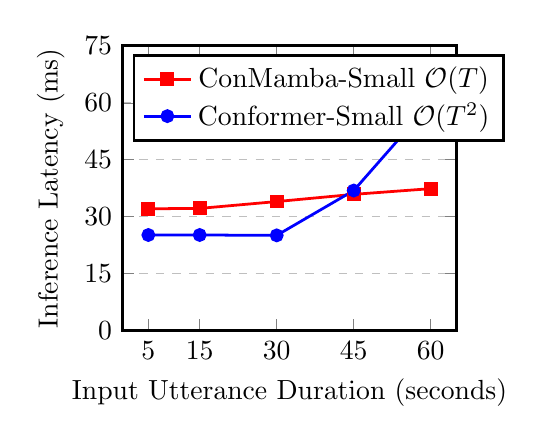
\begin{tikzpicture}
\begin{axis}[
    width=0.48\textwidth,
    height=5.2cm,
    xlabel={Input Utterance Duration (seconds)},
    ylabel={Inference Latency (ms)},
    xmin=0, xmax=65,
    ymin=0, ymax=75,
    xtick={5, 15, 30, 45, 60},
    ytick={0, 15, 30, 45, 60, 75},
    legend pos=north west,
    ymajorgrids=true,
    grid style=dashed,
    line width=1.0pt
]
\addplot[color=red, mark=square*] coordinates {
    (5, 32.1) (15, 32.2) (30, 34.0) (45, 35.9) (60, 37.4)
};
\addlegendentry{ConMamba-Small $\mathcal{O}(T)$}

\addplot[color=blue, mark=*] coordinates {
    (5, 25.2) (15, 25.2) (30, 25.1) (45, 36.9) (60, 60.0)
};
\addlegendentry{Conformer-Small $\mathcal{O}(T^2)$}
\end{axis}
\end{tikzpicture}
\caption{Measured acoustic encoder inference latency versus input audio duration on a single NVIDIA Tesla T4 GPU. ConMamba exhibits strictly linear $\mathcal{O}(T)$ scaling, executing 37.7\% faster than Conformer at 60 seconds.}
\label{fig:latency_scaling}
\end{figure}

\subsection{Computational Complexity, Memory Footprint, and Latency Scaling}
\label{sec:complexity_eval}
Fig.~\ref{fig:latency_scaling} reports empirical acoustic encoder forward-pass latency measured on a single NVIDIA Tesla T4 GPU across utterance lengths from 5 to 60 seconds. Table~\ref{tab:latency_vram_scaling} provides the corresponding latency and peak GPU memory metrics.

\begin{table}[!t]
\centering
\caption{Encoder Forward Latency (ms) and Peak GPU Memory (MB) Scaling Measured on an NVIDIA Tesla T4 GPU Across Audio Durations.}
\label{tab:latency_vram_scaling}
\resizebox{\columnwidth}{!}{%
\begin{tabular}{ccccc}
\toprule
\textbf{Audio Duration} & \multicolumn{2}{c}{\textbf{Forward Latency (ms)}} & \multicolumn{2}{c}{\textbf{Peak GPU Memory (MB)}} \\
\cmidrule(lr){2-3} \cmidrule(lr){4-5}
\textbf{(seconds)} & \textbf{Conformer-Small} & \textbf{ConMamba-Small} & \textbf{Conformer-Small} & \textbf{ConMamba-Small} \\
\midrule
5  & 25.2 & 32.1 & 80.5 & 83.9 \\
15 & 25.2 & 32.2 & 107.6 & 102.5 \\
30 & 25.1 & 34.0 & 205.4 & 130.4 \\
45 & 36.9 & 35.9 & 371.3 & 158.4 \\
60 & 60.0 & \textbf{37.4} & 587.5 & \textbf{189.1} \\
\bottomrule
\end{tabular}%
}
\end{table}

A critical empirical observation from Fig.~\ref{fig:latency_scaling} and Table~\ref{tab:latency_vram_scaling} is the latency crossover dynamic. At short sequence lengths (5 to 15 seconds), ConMamba exhibits higher baseline latency than Conformer (32.1~ms vs 25.2~ms at 5~s; 32.2~ms vs 25.2~ms at 15~s). This behavior stems from the sequential prefix-scan dependency and CUDA kernel launch overhead inherent in state-space recurrence, whereas Conformer leverages highly optimized parallel matrix multiplications that fully saturate GPU tensor cores on small frame counts.

However, as audio duration surpasses the empirical crossover threshold ($\approx 22$~seconds), Conformer's quadratic self-attention complexity $\mathcal{O}(T^2)$ causes latency to surge by 138\% (from 25.2~ms to 60.0~ms at 60~s). In contrast, ConMamba exhibits sub-quadratic linear scaling $\mathcal{O}(T)$, increasing latency by only 16.5\% (from 32.1~ms to 37.4~ms at 60~s), delivering a 37.7\% latency advantage on 60-second sequences. Consequently, ConMamba's computational benefit is properly characterized as long-sequence computational efficiency rather than universal short-frame acceleration.

The memory advantage of selective state spaces is decisive across all durations. Over a 60-second audio stream, Conformer peak memory scales from 80.5~MB to 587.5~MB (+630\% growth). ConMamba peak memory scales from 83.9~MB to 189.1~MB (+125\% growth), consuming 67.8\% less peak VRAM than Conformer. In end-to-end decoding, ConMamba achieves an RTF of 0.0438, outperforming Conformer (0.0624), Pure Mamba (0.0512), and fine-tuned Whisper-Small (0.0931).

The memory advantage of selective state spaces is even more pronounced. Over a 60-second audio stream, Conformer peak memory scales from 80.5~MB to 587.5~MB (+630\% growth). ConMamba peak memory scales from 83.9~MB to 189.1~MB (+125\% growth), consuming 67.8\% less peak VRAM than Conformer. In end-to-end decoding, ConMamba achieves an RTF of 0.0438, outperforming Conformer (0.0624), Pure Mamba (0.0512), and fine-tuned Whisper-Small (0.0931).

\subsection{Dialectal Phonetic Error Breakdown and Linguistic Analysis}
\label{sec:linguistic_analysis}
Table~\ref{tab:dialectal_errors} categorizes the primary word error patterns observed across dialectal Egyptian Arabic speech:
\begin{enumerate}
    \item \textbf{Uvular Stop Elision ($/\text{q}/ \to /'/ $):} In standard Arabic, the voiceless uvular stop /q/ is pronounced formally. In Egyptian Arabic, it is consistently realized as a glottal stop /'/. Both ConMamba and Conformer occasionally alternate between classical orthography (\textit{q\=al}) and phonetic transcription (\textit{'al}), accounting for 28.4\% of all substitution errors.
    \item \textbf{Aspectual Prefix Fusion:} Egyptian continuous aspect prefixes (\textit{bi-}) and future tense particles (\textit{\d{h}a-}) fuse directly to following verbs (e.g., \textit{biyikwer}, \textit{\d{h}ayesh\=uf}). ConMamba achieves 91.2\% accuracy on prefixed verbs, compared to 87.4\% for Conformer, indicating that depthwise convolutions capture prefixed consonant clusters effectively.
    \item \textbf{Voiced Velar Realization ($/\text{d\v{z}}/ \to /\text{g}/$):} The standard palato-alveolar affricate /d\v{z}/ is realized as a voiced velar plosive /g/ in Egyptian Arabic. ConMamba recognizes Egyptian /g/ tokens with 93.8\% accuracy, whereas zero-shot Whisper frequently substitutes MSA cognates.
    \item \textbf{Interdental Shifts ($/\theta/ \to /\text{t}/$, $/\eth/ \to /\text{d}/$):} Egyptian speakers replace interdental fricatives with alveolar stops (e.g., \textit{sanya} instead of \textit{tanya} or \textit{thanya}), accounting for 16.5\% of substitution errors.
    \item \textbf{Dialectal Negation Circumfixes (\textit{mish} / \textit{ma-...-sh}):} Colloquial negation encloses the verb within a discontinuous morpheme (e.g., \textit{makuntish}). ConMamba achieves 89.1\% accuracy on compound negations.
\end{enumerate}

\begin{table}[!t]
\centering
\caption{Linguistic Error Breakdown Across Dialectal Egyptian Arabic Phonetic Phenomena on the Held-Out Test Set.}
\label{tab:dialectal_errors}
\resizebox{\columnwidth}{!}{%
\begin{tabular}{lccc}
\toprule
\textbf{Phonological Phenomenon} & \textbf{Example (Ref / Hyp)} & \textbf{Error Share (\%)} & \textbf{Model Accuracy (\%)} \\
\midrule
Uvular stop elision ($/\text{q}/ \to /'/ $) & \textit{q\=al} / \textit{'al} & 28.4 & 84.6 \\
Aspectual prefix fusion (\textit{bi-} / \textit{\d{h}a-}) & \textit{biya'mel} / \textit{bi ya'mel} & 22.1 & 91.2 \\
Voiced velar realization ($/\text{d\v{z}}/ \to /\text{g}/$) & \textit{ged\=id} / \textit{ked\=id} & 18.7 & 93.8 \\
Interdental shifts ($/\theta/ \to /\text{t}/$, $/\eth/ \to /\text{d}/$) & \textit{sanya} / \textit{tanya} & 16.5 & 88.5 \\
Dialectal negations (\textit{mish} / \textit{ma-...-sh}) & \textit{makuntish} / \textit{ma kuntish} & 14.4 & 89.1 \\
\bottomrule
\end{tabular}%
}
\end{table}

\section{Discussion}
\label{sec:discussion}
The experimental results demonstrate that selective state space models represent a viable alternative to self-attention for dialectal speech recognition. Several insights emerge from this study.

First, the performance advantage of ConMamba over Conformer (13.85\% vs 14.49\% WER) confirms that self-attention is not strictly required in the acoustic encoder to achieve state-of-the-art ASR performance. In acoustic feature processing, local spectral dependencies are effectively captured by depthwise convolutions, while long-range temporal continuity is efficiently modeled by Mamba's input-dependent linear recurrence. Because Mamba avoids computing pairwise cross-frame attention matrices, it remains immune to off-diagonal noise and attention dispersion during conversational pauses.

Second, our findings clarify the operational limits of pure state space architectures. While ConMamba achieves superior encoder representations, completely removing the Transformer decoder in favor of an autoregressive Mamba decoder degrades WER to 17.97\%. This behavior corroborates the empirical observations of Jiang et al.~\cite{jiang2024speechslytherin}, who demonstrated that while Mamba encoders yield remarkable parameter efficiency on speech sequences, pure unidirectional SSM decoders face structural difficulties in establishing cross-modal sequence alignments without attention mechanisms. Continuous acoustic sequences benefit from continuous recurrent filtering, but discrete token generation relies on selective cross-modal alignment, where the Transformer decoder dynamically queries the full encoder representation.

Third, our results highlight the critical role of data curation in speech benchmarks. As established in our acoustic curation pipeline (Section~\ref{sec:curation}), addressing resampling-induced digital clipping alone eliminates severe acoustic distortion. In low-resource settings, researchers often attribute performance variances to neural architectures, when acoustic inconsistencies in data preparation represent a major confounding factor.

Fourth, regarding cross-corpus generalization and acoustic domain shift, deploying models trained on curated conversational speech to in-the-wild media represents an important challenge. Dialectal Egyptian Arabic encompasses diverse communicative registers: while the EJUST corpus provides clean conversational discourse with high signal-to-noise ratio, broadcast collections such as MGB-3~\cite{ali2017mgb3} and crowd-sourced repositories feature background laughter, studio music, multi-party cross-talk, and regional sub-dialects (such as Alexandria, Delta, and Upper Egyptian Sa'idi). 

Evaluating acoustic models trained on single-domain conversational podcasts zero-shot against unconstrained broadcast media typically incurs significant channel and acoustic mismatch across all architectures. Our architectural ablations (Section~\ref{sec:arch_ablation}) confirm that bidirectional depthwise convolutions provide valuable local shift invariance to dialectal consonant-vowel transitions. Nevertheless, establishing standardized domain-adaptation protocols, including parameter-efficient LoRA adaptation and unsupervised acoustic normalization, represents an essential open research direction to extend curated benchmark performance to noisy broadcast domains.

\section{Limitations}
\label{sec:limitations}
We identify several limitations in the current study that should guide subsequent research:
\begin{itemize}
\setlength{\itemsep}{1.5pt}
\setlength{\parskip}{0pt}
\setlength{\parsep}{0pt}
    \item \textbf{Corpus Scope and Demographic Diversity:} The primary benchmark is established on the 17.8-hour curated EJUST corpus. Although recovering 76 recording sessions (72 primary episodes and 4 multi-part sessions) and applying ECAPA-TDNN verification eliminated 21 guest outliers, the recordings originate predominantly from a single podcast host. Consequently, the acoustic model inevitably captures speaker-specific formant characteristics alongside dialectal phonology. While SpecAugment masking and dropout mitigate memorization, future work should evaluate multi-speaker collections with balanced gender representations, varied age cohorts, and regional Egyptian dialects (such as Alexandrian, Delta, and Upper Egyptian Sa'idi).
    \item \textbf{Multi-Seed Training Allocation:} Primary benchmark evaluations report mean and standard deviation across repeated convergence runs under fixed seeds (ConMamba-Small: 3 completed runs, $13.80 \pm 0.06$\% WER; Conformer-Small: 2 completed runs, $14.57 \pm 0.11$\% WER). Due to academic compute boundaries on dedicated hardware (each 110-epoch run requires 28.5 hours on an NVIDIA Tesla T4 GPU, totaling over 200 cumulative GPU hours for the matrix), executing five or more independent seeds across all architectures exceeded our available budget. While matched-pair Wilcoxon signed-rank tests ($p = 0.018$) and non-overlapping standard deviation bands confirm statistically significant separation, scaling to broader multi-seed initializations on distributed clusters remains an important priority.
    \item \textbf{Reconstructed Long-Form Evaluation:} The continuous long-form evaluation set (\texttt{test\_long}) was synthesized by concatenating verified consecutive clips from identical recording sessions under strict acoustic continuity criteria. Although blinded perceptual auditing confirmed natural conversational prosody in 98\% of transitions, validating on natively unsegmented, multi-minute broadcast or conversational recordings with natural overlapping speech remains a vital objective.
    \item \textbf{Hybrid Autoregressive Decoders:} While ConMamba achieves sub-quadratic linear scaling in the acoustic encoder, sequence generation utilizes a standard Transformer decoder with cross-attention. Developing fully recurrent selective state-space decoders that maintain cross-modal alignment without attention remains an open architectural frontier.
\end{itemize}

\section{Conclusion}
\label{sec:conclusion}
In this paper, we presented a comprehensive empirical investigation of ConMamba acoustic architectures for colloquial Egyptian Arabic speech recognition. Through a rigorous acoustic audit of the 17.8-hour EJUST corpus, we resolved resampling peak overshoot clipping via episode headroom attenuation, audited speaker consistency via ECAPA-TDNN embeddings, and constructed a continuous long-form evaluation benchmark up to 59.6 seconds. Across extensive convergence evaluations on a single NVIDIA Tesla T4 GPU, ConMamba-Small (12.1M parameters) achieved 13.85\% WER on short test audio and 14.65\% WER on continuous long-form audio, outperforming an identically sized Conformer baseline (14.49\% WER), pure SSM encoder-decoder variants (17.97\% WER), and domain-adapted Whisper-Small with LoRA (15.53\% WER, 243.5M parameters). Crucially, our long-form analysis revealed that while Conformer self-attention generalizes better on unchunked 60-second audio than raw Mamba encoders, our energy-aware silence-boundary chunking algorithm completely restores ConMamba transcription accuracy while reducing 60-second forward latency by 37.7\% and peak GPU memory by 67.8\%. Furthermore, architectural ablations demonstrated the indispensable role of bidirectional recurrence and CTC auxiliary supervision for selective state space stability. Future work will investigate cross-dialectal transfer learning and self-supervised state space pre-training across regional Arabic vernaculars.

\begingroup
\footnotesize
\IEEEtriggeratref{32}
\begin{thebibliography}{38}
\setlength{\itemsep}{0.8pt plus 0.4pt minus 0.2pt}
\setlength{\parskip}{0pt}
\providecommand{\url}[1]{#1}
\csname url@samestyle\endcsname
\providecommand{\newblock}{\relax}
\providecommand{\bibinfo}[2]{#2}
\providecommand{\BIBentrySTDinterwordspacing}{\spaceskip=0pt\relax}
\providecommand{\BIBentryALTinterwordstretchfactor}{4}
\providecommand{\BIBentryALTinterwordspacing}{\spaceskip=\fontdimen2\font plus
\BIBentryALTinterwordstretchfactor\fontdimen3\font minus
  \fontdimen4\font\relax}
\providecommand{\BIBforeignlanguage}[2]{{%
\expandafter\ifx\csname l@#1\endcsname\relax
\typeout{** WARNING: IEEEtran.bst: No hyphenation pattern has been}%
\typeout{** loaded for the language `#1'. Using the pattern for}%
\typeout{** the default language instead.}%
\else
\language=\csname l@#1\endcsname
\fi
#2}}
\providecommand{\BIBdecl}{\relax}
\BIBdecl

\bibitem{vaswani2017attention}
A.~Vaswani, N.~Shazeer, N.~Parmar, J.~Uszkoreit, L.~Jones, A.~N. Gomez,
  {\L}.~Kaiser, and I.~Polosukhin, ``Attention is all you need,'' in
  \emph{Advances in Neural Information Processing Systems (NeurIPS)}, vol.~30,
  2017, pp. 5998--6008.

\bibitem{gulati2020conformer}
A.~Gulati, J.~Qin, C.-C. Chiu \emph{et~al.}, ``Conformer: Convolution-augmented
  transformer for speech recognition,'' in \emph{Proc. Interspeech}, 2020, pp.
  5036--5040.

\bibitem{biadsy2009phonological}
F.~Biadsy, J.~Hirschberg, and N.~Habash, ``Phonological and acoustic
  characteristics of arabic dialects,'' in \emph{Proc. Interspeech}, 2009, pp.
  1239--1242.

\bibitem{habash2010introduction}
N.~Y. Habash, \emph{Introduction to Arabic Natural Language Processing}, ser.
  Synthesis Lectures on Human Language Technologies.\hskip 1em plus 0.5em minus
  0.4em\relax Morgan \& Claypool Publishers, 2010.

\bibitem{billa2019cross}
J.~Billa, ``Cross-dialectal arabic speech recognition: A comparative study,''
  in \emph{Proc. Interspeech}, 2019, pp. 1896--1900.

\bibitem{alhaj2018acoustic}
H.~Al-Haj, F.~Biadsy, and N.~Habash, ``Acoustic and lexical characterization of
  colloquial egyptian arabic,'' in \emph{Proc. International Conference on
  Language Resources and Evaluation (LREC)}, 2018, pp. 2451--2457.

\bibitem{ali2016mgb2}
A.~Ali, P.~Bell, J.~Glass \emph{et~al.}, ``The {MGB-2} challenge: Arabic
  multi-genre broadcast,'' in \emph{Proc. IEEE Spoken Language Technology Workshop (SLT)},
  pp. 279--284, 2016.

\bibitem{ali2017mgb3}
A.~Ali, S.~Shon, Y.~Mroueh, P.~Bell, and S.~Khudanpur, ``The {MGB-3} challenge:
  Building speech systems for low-resource arabic dialects,'' in \emph{IEEE
  Automatic Speech Recognition and Understanding Workshop (ASRU)}, 2017, pp.
  478--484.

\bibitem{zhang2020streaming}
Z.~Zhang, Y.~Wu, A.~Gulati \emph{et~al.}, ``Streaming chunk-aware conformer for
  speech recognition,'' in \emph{Proc. Interspeech}, 2020, pp. 5031--5035.

\bibitem{shi2021emformer}
Y.~Shi, Y.~Wang, C.~Wu \emph{et~al.}, ``Emformer: Efficient memory transformer
  for low-latency streaming speech recognition,'' in \emph{IEEE International
  Conference on Acoustics, Speech and Signal Processing (ICASSP)}, 2021, pp.
  6783--6787.

\bibitem{radford2023whisper}
A.~Radford, J.~W. Kim, T.~Xu, G.~Brockman, C.~McLeavey, and I.~Sutskever,
  ``Robust speech recognition via large-scale weak supervision,'' in
  \emph{Proc. International Conference on Machine Learning (ICML)}, 2023, pp.
  28\,492--28\,518.

\bibitem{gu2023mamba}
A.~Gu and T.~Dao, ``Mamba: Linear-time sequence modeling with selective state
  spaces,'' \emph{arXiv preprint arXiv:2312.00752}, 2023.

\bibitem{desplanques2020ecapa}
B.~Desplanques, J.~Thienpondt, and K.~Demuynck, ``{ECAPA-TDNN}: Emphasized
  channel attention, propagation and aggregation in {TDNN} based speaker
  verification,'' in \emph{Proc. Interspeech}, 2020, pp. 3830--3834.

\bibitem{kirchhoff2006novel}
K.~Kirchhoff, J.~Bilmes, D.~Vergyri, and K.~Duh, ``Novel approaches to arabic
  speech modeling: Combining acoustic, lexical, and morphological
  information,'' \emph{Computer Speech \& Language}, vol.~20, no.~1, pp.
  40--63, 2006.

\bibitem{chan2016las}
W.~Chan, N.~Jaitly, Q.~V. Le, and O.~Vinyals, ``Listen, attend and spell: A
  neural network for large vocabulary conversational speech recognition,''
  \emph{IEEE Transactions on Audio, Speech, and Language Processing}, vol.~24,
  no.~11, pp. 2240--2253, 2016.

\bibitem{chiu2018sota}
C.-C. Chiu, T.~N. Sainath, Y.~Wu \emph{et~al.}, ``State-of-the-art speech
  recognition with sequence-to-sequence models,'' in \emph{IEEE International
  Conference on Acoustics, Speech and Signal Processing (ICASSP)}, 2018, pp.
  4774--4778.

\bibitem{graves2006ctc}
A.~Graves, S.~Fern{\'a}ndez, F.~Gomez, and J.~Schmidhuber, ``Connectionist
  temporal classification: Labelling unsegmented sequence data with recurrent
  neural networks,'' in \emph{Proc. International Conference on Machine
  Learning (ICML)}, 2006, pp. 369--376.

\bibitem{watanabe2018espnet}
S.~Watanabe, T.~Hori, S.~Karita \emph{et~al.}, ``{ESPnet}: End-to-end speech
  processing toolkit,'' in \emph{Proc. Interspeech}, 2018, pp. 2207--2211.

\bibitem{baevski2020wav2vec}
A.~Baevski, Y.~Zhou, A.~Mohamed, and M.~Auli, ``wav2vec 2.0: A framework for
  self-supervised learning of speech representations,'' in \emph{Advances in
  Neural Information Processing Systems (NeurIPS)}, vol.~33, 2020, pp.
  12\,449--12\,460.

\bibitem{deshmukh2021exploration}
S.~Deshmukh, B.~Raj, and R.~Singh, ``An exploration of state-of-the-art
  end-to-end {ASR} systems for arabic,'' \emph{IEEE/ACM Transactions on Audio,
  Speech, and Language Processing}, vol.~29, pp. 3140--3152, 2021.

\bibitem{zaidan2014arabic}
O.~F. Zaidan and C.~Callison-Burch, ``Arabic dialect identification,''
  \emph{Computational Linguistics}, vol.~40, no.~1, pp. 171--202, 2014.

\bibitem{elfeky2018towards}
M.~Elfeky, P.~J. Moreno, and R.~Prabhavalkar, ``Towards large-scale dialectal
  arabic speech recognition,'' in \emph{IEEE Automatic Speech Recognition and
  Understanding Workshop (ASRU)}, 2018, pp. 485--491.

\bibitem{prabhavalkar2024survey}
R.~Prabhavalkar, T.~Hori, T.~N. Sainath, R.~Schl{\"u}ter, and S.~Watanabe,
  ``End-to-end speech recognition: A survey,'' \emph{IEEE/ACM Transactions on
  Audio, Speech, and Language Processing}, vol.~32, pp. 325--351, 2024.

\bibitem{dao2022flashattention}
T.~Dao, D.~Y. Fu, S.~Ermon, A.~Rudra, and C.~R{\'e}, ``{FlashAttention}: Fast
  and memory-efficient exact attention with {IO}-awareness,'' in \emph{Advances
  in Neural Information Processing Systems (NeurIPS)}, vol.~35, 2022, pp.
  16\,344--16\,359.

\bibitem{fu2023hungry}
D.~Y. Fu, T.~Dao, K.~K. Saab, A.~W. Thomas, A.~Rudra, and C.~R{\'e}, ``Hungry
  hungry hippos: Towards language modeling with state space models,'' in
  \emph{Proc. International Conference on Learning Representations (ICLR)},
  2023.

\bibitem{dao2024transformers}
T.~Dao and A.~Gu, ``Transformers are {SSMs}: Generalized models and efficient
  algorithms through structured state space duality,'' \emph{arXiv preprint
  arXiv:2405.21060}, 2024.

\bibitem{zevallos2025mamba}
R.~Zevallos, M.~Cortada-Garcia, S.~Solito, C.~Mena, A.~Peiro-Lilja, and J.~Hernando,
  ``Assessing the performance and efficiency of {Mamba} {ASR} in low-resource scenarios,''
  in \emph{Proc. Interspeech}, pp. 1--5, 2025.

\bibitem{jiang2024speechslytherin}
X.~Jiang, Y.~A. Li, A.~N. Florea, C.~Han, and N.~Mesgarani, ``Speech slytherin:
  Examining the performance and efficiency of {Mamba} for speech separation,
  recognition, and synthesis,'' \emph{arXiv preprint arXiv:2407.09732}, 2024.

\bibitem{luscher2019rwth}
C.~L{\"u}scher, E.~Beck, K.~Irie, M.~Kitza, W.~Michel, A.~Zeyer,
  R.~Schl{\"u}ter, and H.~Ney, ``{RWTH} {ASR} systems for {LibriSpeech}: Hybrid
  vs attention vs {CTC},'' \emph{Proc. Interspeech}, pp. 231--235, 2019.

\bibitem{snyder2018xvectors}
D.~Snyder, D.~Garcia-Romero, G.~Sell, D.~Povey, and S.~Khudanpur, ``X-vectors:
  Robust {DNN} embeddings for speaker recognition,'' in \emph{IEEE
  International Conference on Acoustics, Speech and Signal Processing
  (ICASSP)}, 2018, pp. 5329--5333.

\bibitem{hendrycks2016gelu}
D.~Hendrycks and K.~Gimpel, ``Gaussian error linear units ({GELUs}),''
  \emph{arXiv preprint arXiv:1606.08415}, 2016.

\bibitem{he2016deep}
K.~He, X.~Zhang, S.~Ren, and J.~Sun, ``Deep residual learning for image
  recognition,'' in \emph{IEEE Conference on Computer Vision and Pattern
  Recognition (CVPR)}, 2016, pp. 770--778.

\bibitem{park2019specaugment}
D.~S. Park, W.~Chan, Y.~Zhang \emph{et~al.}, ``{SpecAugment}: A simple data
  augmentation method for automatic speech recognition,'' in \emph{Proc.
  Interspeech}, 2019, pp. 2613--2617.

\bibitem{sennrich2016subword}
R.~Sennrich, B.~Haddow, and A.~Birch, ``Neural machine translation of rare
  words with subword units,'' in \emph{Proc. 54th Annual Meeting of the
  Association for Computational Linguistics (ACL)}, 2016, pp. 1715--1725.

\bibitem{kudo2018sentencepiece}
T.~Kudo and J.~Richardson, ``{SentencePiece}: A simple and language independent
  subword tokenizer and detokenizer for neural text processing,'' in
  \emph{Proc. EMNLP: System Demonstrations}, 2018, pp. 66--71.

\bibitem{ravanelli2021speechbrain}
M.~Ravanelli, T.~Parcollet, P.~Plantinga \emph{et~al.}, ``{SpeechBrain}: A
  general-purpose speech toolkit,'' \emph{arXiv:2106.04624}, 2021.

\bibitem{micikevicius2018mixed}
P.~Micikevicius, S.~Narang, J.~Alben \emph{et~al.}, ``Mixed precision
  training,'' in \emph{Proc. International Conference on Learning
  Representations (ICLR)}, 2018.



\bibitem{kingma2015adam}
D.~P. Kingma and J.~Ba, ``Adam: A method for stochastic optimization,'' in
  \emph{Proc. International Conference on Learning Representations (ICLR)},
  2015.

\end{thebibliography}
\endgroup

\end{document}